\subsection{Das Gehäuse}
\label{subsec:HW:Gehaeuse}
Damit die Wetterstation gebraucht werden kann, muss das PCB vor den Wettereinflüssen geschützt werden. In Absprache mit dem Auftraggeber soll als Wunschziel ein provisorisches Design des Gehäuses erfolgen und dieses mit einem 3D-Drucker gedruckt werden um bei der Bachelor-Thesis Ausstellung am 16. August 2019 ein anschauliches Modell zu haben. Im folgenden Unterkapitel wird aufgezeigt, auf was beim Design des Gehäuses acht gegeben werden muss und in einem folgenden Unterkapitel wird das Design für das provisorische Gehäuse vorgestellt.

\subsubsection{Wichtige Merkmale}
Damit beim Design des Gehäuses nichts vergessen geht, werden hier die wichtigsten Punkte, auf die acht gegeben werden muss, erläutert. Die grobe Dimensionierung wird durch das PCB vorgegeben und ist in Abbildung \ref{fig:Dimensionen1} zu sehen.

\begin{figure}[h]
\centering
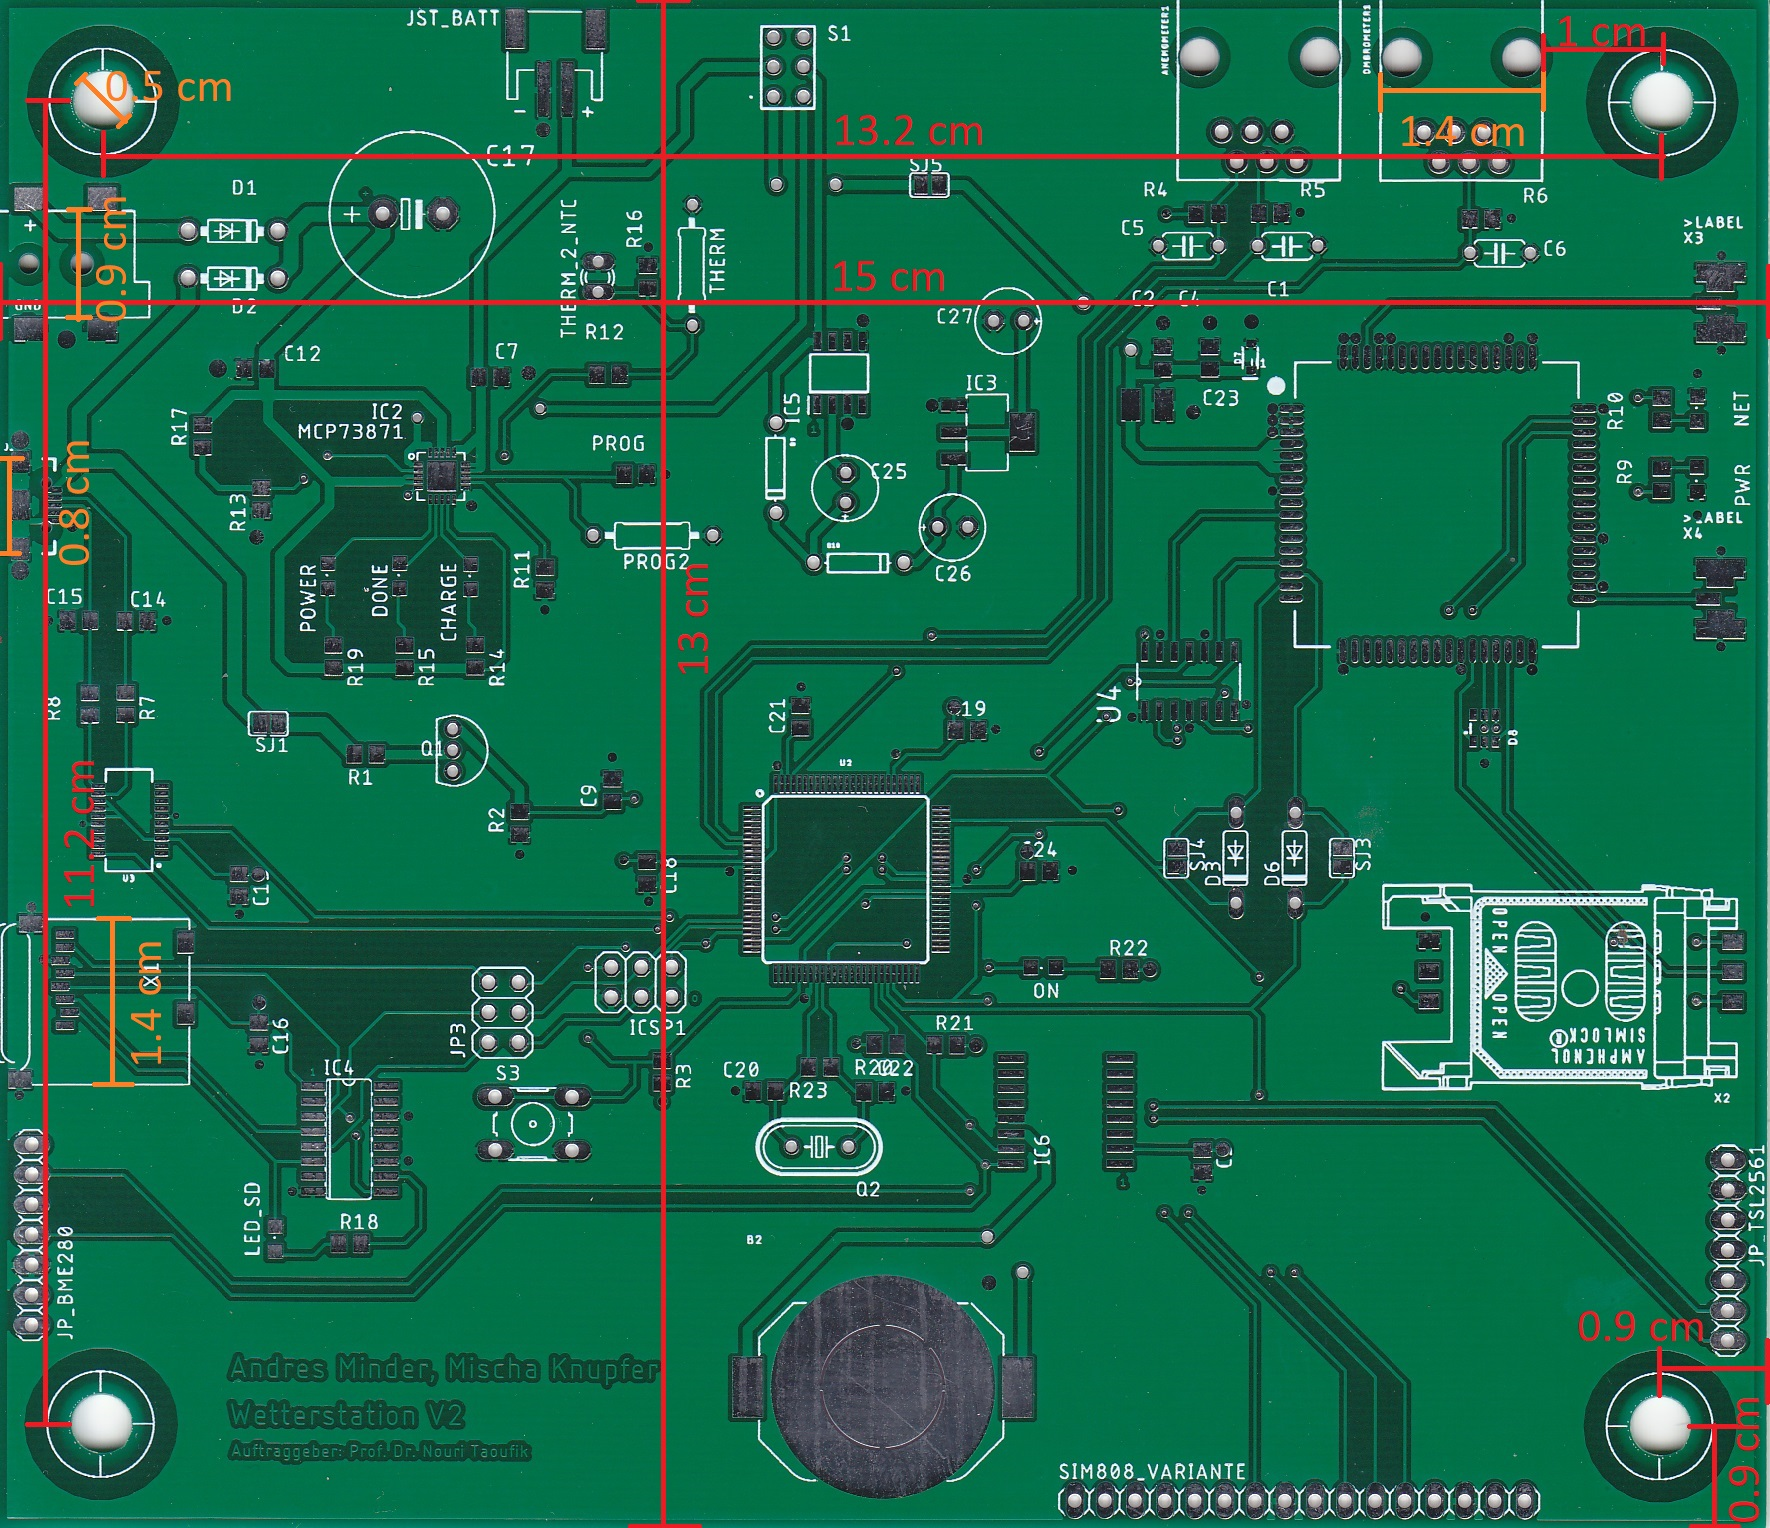
\includegraphics[width=0.9\linewidth]{graphics/Gehaeuse/PCB_Dimensionen.jpg}
\caption{Das noch unbestückte PCB mit den wichtigsten Dimensionen.}
\label{fig:Dimensionen1}
\end{figure}
\newpage
Abbildung \ref{fig:Dimensionen1} zeigt das noch unbestückte PCB, wie es schon in der Hardware Übersicht verwendet wurde, mit den wichtigsten Dimensionen. Das PCB hat eine Breite von 15cm, eine länge von 13cm. Die Mittelpunkte der 5mm breiten Bohrlöcher sind 13.2cm weit entfernt in der Breite und 11.2cm in der Länge, wobei diese jeweils 9mm vom Rand entfernt sind. Die Breite der Bauteile die aus dem Gehäuse hinausragen sind 1.4cm (RJ11, $\mu$SD), 0.9cm (DCIN Jack) und 0.8cm ($\mu$USB). Damit alle Bauteile von der Höhe her Platz haben, muss das Gehäuse nach oben hin mindestens über 3cm Freiraum verfügen wegen dem zum MCP73871 gehörenden Elektroly-Kondensator (C17). Der Akkumulator soll ebenfalls im Gehäuse Platz finden, weshalb genügend Platz (min. 2cm) in der Tiefe für diesen zur Verfügung stehen muss. Da es eine Bestückungsvariante gibt für den SIM808, soll das Gehäuse an der unteren Seite um mindestens 4cm erweitert werden, da das Breakout Board des SIM808 ansonsten nicht angeschlossen werden kann. Auf der rechten Seite werden Antennen für den SIM808 angeschlossen, weshalb das Gehäuse auf dieser Seite um mindestens 1cm erweitert werden soll, damit diese nicht knicken. Ebenfalls sollen auch die Kabel des Akkumulators vom knicken geschützt werden, hier benötigt man eine erweiterung des Gehäuses von mindestens 3mm, da die Kabel selbst eine höhere Flexibilität als die Antennen aufweisen. Auf der linken Seite befindet sich die $\mu$USB-Buchse, sowie die Öffnung für die $\mu$SD-Karte. Diese Öffnungen ragen ein wenig hinaus und sollten gut geschützt werden, weshalb eine Erweiterung der Dimensionierung auf der Linken Seite von 1mm empfohlen ist. Äusserst wichtig ist ebenfalls, dass der BME280 auf der linken Seite des Gehäuses nach aussen gebracht wird und in einem gut mit Aussenluft durchströmten eigenen Raum seinen Platz findet. Der TSL2561 wird ebenfalls auf der rechten Seite nach aussen geführt, damit dieser dort unter einem mit durchsichtigem Plexiglas versehenen eigenen Raum die Lichtintensität messen kann.\\[0.5cm]
Die wichtigsten Punkte wurden erläutert, weshalb es nun zum Design des Gehäuses kommt, welches im nächsten Abschnitt vorgestellt wird.

\subsubsection{Das Design}
Im vorhergehenden Unterkapitel wurden die wichtigsten Merkmale und Dimensionen des Gehäuses erläutert. In diesem Unterkapitel wird nun das provisorische Design vorgestellt. Da für den Zusammenbau das PCB auf einen Teil des Gehäuses gelegt wird und mit einem zweiten Teil überdeckt, wird in diesem Abschnitt der Begriff \textit{Boden} für den unteren Teil und \textit{Deckel} für den oberen Teil verwendet. Das Design wurde mit dem CAD-Programm Autodesk Fusion 360 erstellt, welches den Studenten von Bildungseinrichtungen wie der FHNW frei zur Verfügung steht.
\newpage

\begin{figure}[h]
\centering
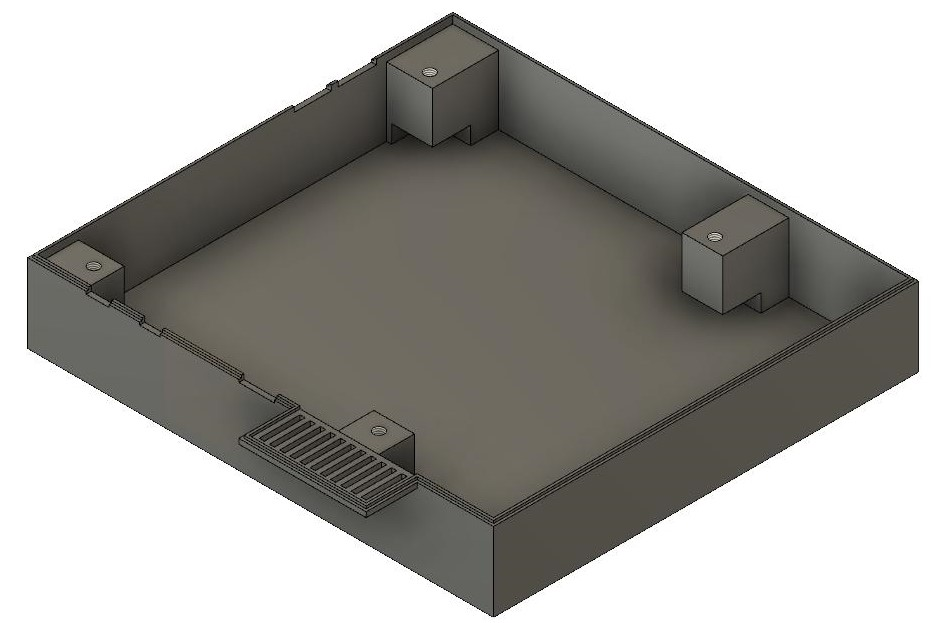
\includegraphics[width=0.99\linewidth]{graphics/Gehaeuse/Design_Boden.jpg}
\caption{Gesamtansicht des Designs des Bodens.}
\label{fig:D:Boden}
\end{figure}

Die Gesamtansicht des Designs des Bodens ist in Abbildung \ref{fig:D:Boden} zu sehen. Diverse Blöcke und Aussparungen sind deutlich zu sehen, worauf mit der Hilfe von den nachfolgenden Abbildungen näher eingegangen wird.\\

{\begin{minipage}[b][8cm][t]{0.39\textwidth}
Das PCB muss erhöht sein, damit der Akku darunter Platz findet. Ausserdem soll eine Schraube das Gehäuse mit dem PCB verbinden. Aus diesen Gründen wurden im Boden Blöcke implementiert, welche ein Schraubengewinde besitzen, wie in Abbildung \ref{fig:D:Boden:Schrauben} ersichtlich ist. Am unteren Ende des Schraubenblocks befindet sich eine Aussparung. Diese Aussparung bietet Platz für eine Mutter, falls das implementierte Gewinde fehlerhaft gedruckt wird.
\end{minipage}}
{\begin{minipage}[b][8cm][t]{0.6\textwidth}
\centering
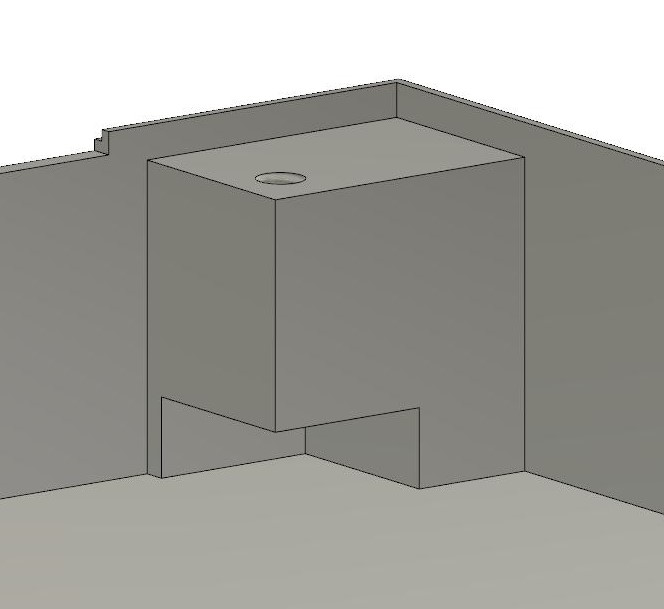
\includegraphics[width=0.8\linewidth]{graphics/Gehaeuse/Design_Boden_Schrauben.jpg}
\captionof{figure}{Design des Schraubenblocks des Bodens.}
\label{fig:D:Boden:Schrauben}
\end{minipage}}

\newpage
\begin{figure}[h]
\centering
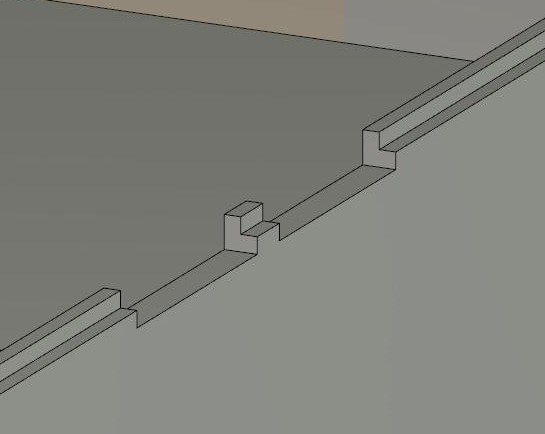
\includegraphics[width=0.5\linewidth]{graphics/Gehaeuse/Design_Boden_Aussparungen.jpg}
\caption{Aussparungen für Bauteile, welche aus dem Gehäuse hinausragen.}
\label{fig:D:Boden:Aussparungen}
\end{figure}
Die in Abbildung \ref{fig:D:Boden:Aussparungen} ersichtlichen Aussparungen sind notwendig um Öffnungen im Gehäuse zu generieren, welche Platz für die hinausragenden Bauteile bieten. Beim Boden sind diese Aussparungen alle gleich tief, da die Bauteile alle auf dem planen PCB angelötet sind und dieses somit als Referenz gilt.

\begin{figure}[h]
\centering
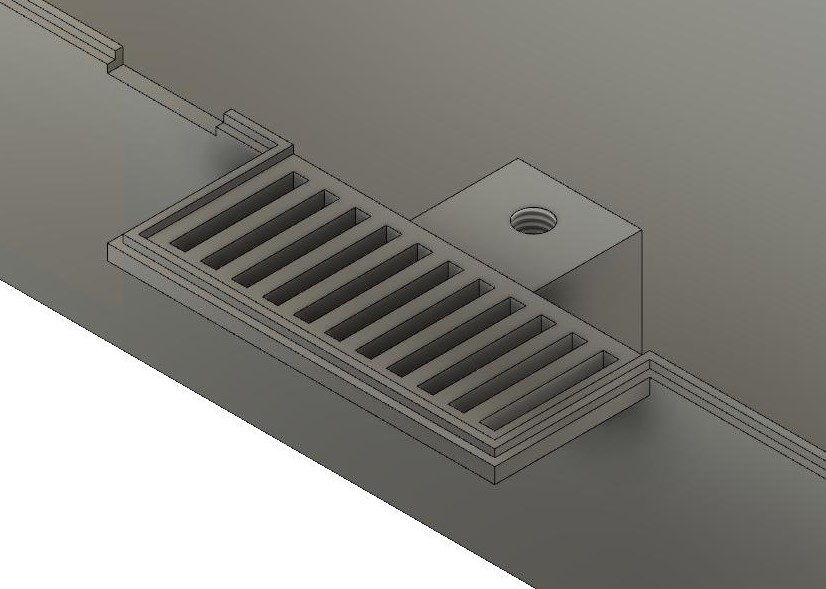
\includegraphics[width=0.7\linewidth]{graphics/Gehaeuse/Design_Boden_BME.jpg}
\caption{Seitenwand für den BME280-Extraraum mit Luftschlitzen.}
\label{fig:D:Boden:BME}
\end{figure}
Der BME280 muss nach aussen geführt werden in einen kleinen Extraraum, welcher gut belüftet ist. Nur so ist der BME280 in der Lage, die exakten Messwerte liefern zu können. Aus diesem Grund wird ein kleiner Extraraum am Rand des Gehäuses gefertigt, welcher mit Luftschlitzen versehen ist. In Abbildung \ref{fig:D:Boden:BME} sieht man den Boden für den im Deckel implementierten Extraraum. Der Boden ist, wie erwähnt, mit 2mm breiten Luftschlitzen versehen.

\newpage

\begin{figure}[h]
\centering
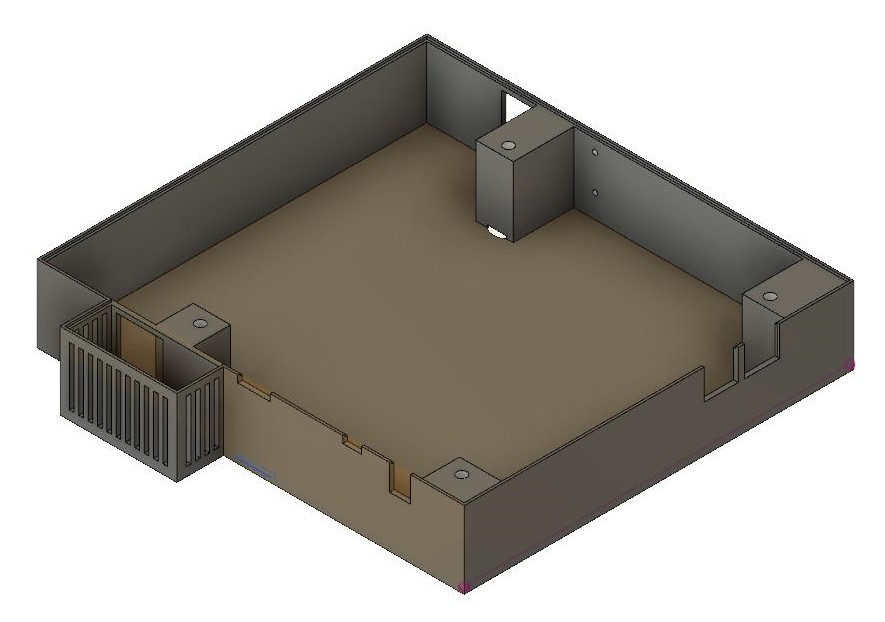
\includegraphics[width=0.99\linewidth]{graphics/Gehaeuse/Design_Deckel.jpg}
\caption{Gesamtansicht des Designs des Deckels.}
\label{fig:D:Deckel}
\end{figure}
Die Gesamtansicht des Designs des Deckels ist in Abbildung \ref{fig:D:Deckel} zu sehen. Wie schon beim Boden sind auch hier diverse Blöcke und Aussparungen zu sehen, auf welche mit der Hilfe von den nachfolgenden Abbildungen näher eingegangen wird.\\

{\begin{minipage}[b][9cm][t]{0.39\textwidth}
Die Schraubenblöcke des Deckels sind weniger interessant, da diese durchgehende Blöcke sind mit einem entsprechenden Gewinde. Aus diesem Grund wurde in Abbildung \ref{fig:D:Deckel:Schrauben} die Aussenseite des Deckels abgebildet, welche die Schraubenversenkung zeigt. In dieser Schraubenversenkung wird der Kopf der verwendeten Schraube seinen Platz finden, weshalb es zu keinem herausragen einer Schraube kommt.
\end{minipage}}
{\begin{minipage}[b][9cm][t]{0.6\textwidth}
\centering
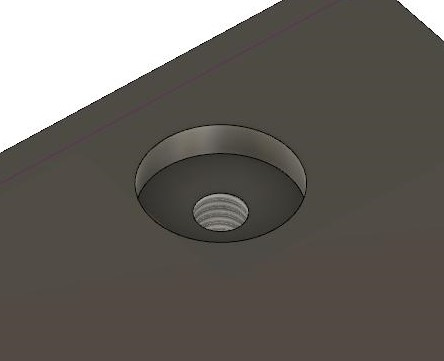
\includegraphics[width=0.8\linewidth]{graphics/Gehaeuse/Design_Deckel_Schraubenversenkung.jpg}
\captionof{figure}{Schraubenversenkung im Deckel.}
\label{fig:D:Deckel:Schrauben}
\end{minipage}

\begin{figure}[h]
\centering
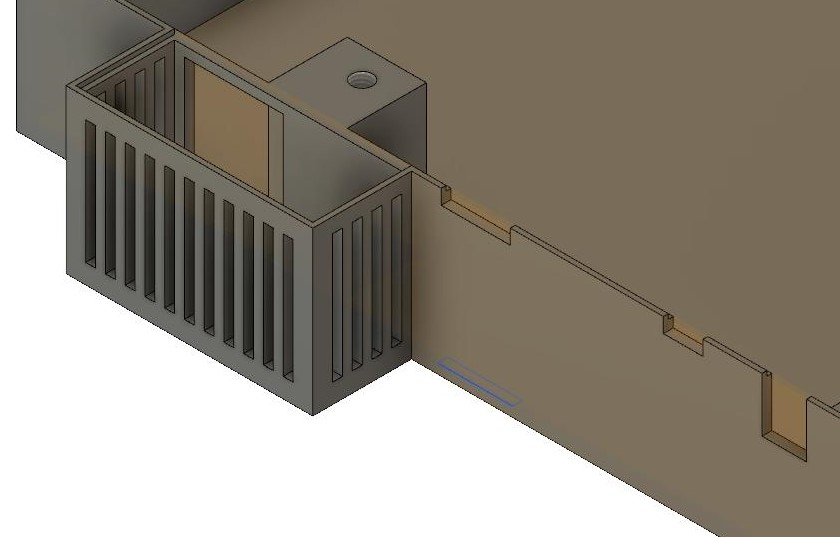
\includegraphics[width=0.6\linewidth]{graphics/Gehaeuse/Design_Deckel_BMEundAussparungen.jpg}
\caption{Aussparungen für Bauteile, welche aus dem Gehäuse hinausragen und der designte Extraraum für den BME280 mit Luftschlitzen.}
\label{fig:D:Deckel:BME}
\end{figure}
Abbildung \ref{fig:D:Deckel:BME} zeigt den bereits erwähnten Extraraum des BME280. Die Luftschlitze sind deutlich zu erkennen und an jeder Seite des Extraraumes angebracht. Ausserdem ist auf dieser Abbildung ebenso ersichtlich, dass die Aussparungen verschiedene Höhen aufweisen. Die Höhe einer Aussparung ist Bauteilabhängig, genauso wie deren Breite.

\begin{figure}[h]
\centering
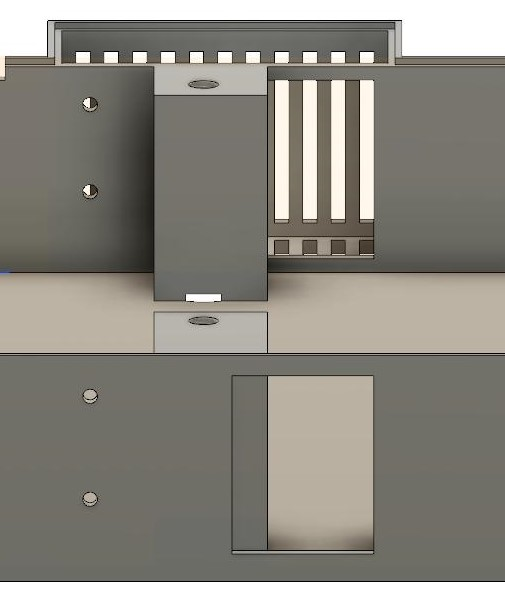
\includegraphics[width=0.5\linewidth]{graphics/Gehaeuse/Design_Deckel_TSL.jpg}
\caption{Öffnung und Bohrungen für den TSL2561 und den BME280.}
\label{fig:D:Deckel:TSL}
\end{figure}
Um den BME280 und den TSL2561 hinausführen zu können, wurden im Gehäuse entsprechende Öffnungen und auch Schraubenlöcher eingelassen. Die eben genannten Öffnungen und Schraubenlöcher sind in Abbildung \ref{fig:D:Deckel:TSL} äusserst gut ersichtlich.
\newpage
{\begin{minipage}[b][6cm][t]{0.49\textwidth}
\centering
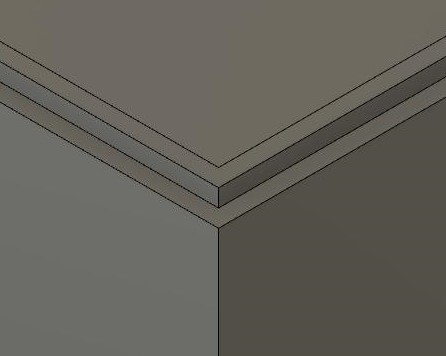
\includegraphics[width=0.8\linewidth]{graphics/Gehaeuse/Design_Boden_Rand.jpg}
\captionof{figure}{Design des Randes vom Boden zum Deckel hin.}
\label{fig:D:Boden:Rand}
\end{minipage}}
{\begin{minipage}[b][6cm][t]{0.49\textwidth}
\centering
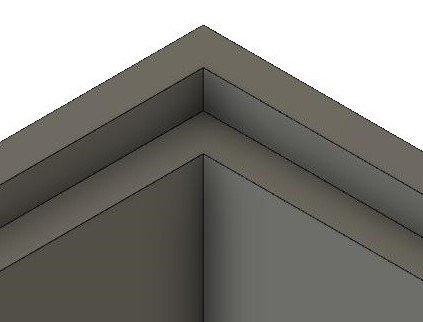
\includegraphics[width=0.8\linewidth]{graphics/Gehaeuse/Design_Deckel_Rand.jpg}
\captionof{figure}{Design des Randes vom Deckel zum Boden hin.}
\label{fig:D:Deckel:Rand}
\end{minipage}}

Damit das Befestigen des Bodens mit dem Deckel einfacher zu handhaben ist, wurde beim Boden die äussere Hälfte des Randes um 1mm gesenkt, wobei beim Deckel die innere Hälfte des Randes um 1mm gesenkt wurde. Dank diesem Feature ist es möglich den Deckel wie ein Puzzlestück am Boden anzubringen, bevor die Verschraubung von statten geht.\\[0.25cm]
Das Design des Gehäuses für das PCB wurde in diesem Unterkapitel näher erläutert. Es sei jedoch erwähnt, dass dieses Gehäuse nicht geeignet ist um die Wetterstation im freien betreiben zu können. Das hier vorgestellte Design zeigt lediglich auf, auf was beim Gehäuse, in Bezug auf das PCB, geachtet werden muss. Damit das Gehäuse für den Gebrauch im freien taugt, muss es zwingend gegen Regen und Staub dicht sein, so dass die verwendete Elektronik keine Schäden erleidet. Dennoch muss der BME280 mit Aussenluft belüftet werden, was bei einem möglichst Regen- und Staubdichten Gehäuse eine zusätzliche, kontrollierte Belüftung notwendig macht. Ausserdem muss auf einen möglichen Hitzestau durch Sonneneinstrahlung getestet und gegebenfalls eine Kühlung integriert werden.

\subsubsection{Probleme mit dem gedruckten Gehäuse}
Das mit einem 3D-Printer gedruckte Gehäuse aus weissem PLA weist Mängel auf. Zum einen kam es durch die Schwingungen des Druckers zu Fehlprints im Bereich des Extraraumes für den BME280, da die Lamellen zu instabil sind (dünn und lang). Das implementierte Gewinde für die Schrauben war unzureichend gedruckt, weshalb es lediglich zu einer Verengung des Schraubenlochs kam und kleinere Schrauben verwendet werden mussten. Zudem hin kommt eine Differenz in der Distanz der Bohrlöcher, denn die Bohrlöcher scheinen wegen 1mm nicht aufeinander zu passen und mussten deshalb aufgebohrt werden. Dies führte dazu, dass am unteren Ende für die Schrauben eine Mutter positioniert und angeklebt werden musste, da die Schrauben sonst keinen Halt fänden. Ebenfalls gab es Probleme beim BME280 und beim TSL2561, weil die auf dem Print implementierten Pinheader mit den Schraubenblocks kollidierten, was ebenfalls mit einer Bohrmaschine behoben wurde. Die Anschlüsse auf der Seite des $\mu$USB-Anschlusses ragten nicht hinaus, weshalb die Öffnung des $\mu$USB-Anschlusses vergrössert werden musste, damit ein Kabel angeschlossen werden kann. Die Schrauben, um den BME280 und den TSL2561 zu befestigen, gab es im OBI nicht zu kaufen, weshalb auf Holzschrauben mit angemessenem Durchmesser zurückgegriffen werden musste und eine Holzleiste für die Befestigung benötigt wurde. Der transparente Raum für den TSL2561 konnte nicht gedruckt werden, da das transparente Filament nicht transparent genug wäre und Rillen enthalten würde, weshalb ein transparentes Stück Plastik einer Verpackung angeklebt wurde. \\[0.25cm]
Die Firmware, die Hardware und das Gehäuse wurden erstellt, weshalb nun die Validierung des Konzepts im nächsten Kapitel folgt.
